\documentclass{beamer}

\usetheme{Boadilla}

%%%%%%%%%%%%%%%%%%%%%%%%%%%%%%%%%%%%%%%%%%%%%%%%%%%%%%%%%%%%%%%%%%%%%%%%%%%%%%%
%% Packages
%%%%%%%%%%%%%%%%%%%%%%%%%%%%%%%%%%%%%%%%%%%%%%%%%%%%%%%%%%%%%%%%%%%%%%%%%%%%%%%

\usepackage[utf8]{inputenc}
\usepackage{minted}
\usepackage{tikz}

\usetikzlibrary{cd}
\usetikzlibrary{fit}
\usetikzlibrary{matrix}

% Shady minted centering stuff
% https://tex.stackexchange.com/questions/161124/how-to-make-a-minted-code-listing-centered-on-a-page
\usepackage{letltxmacro}
\usepackage{xpatch}
\LetLtxMacro{\cminted}{\minted}
\let\endcminted\endminted
\xpretocmd{\cminted}{\RecustomVerbatimEnvironment{Verbatim}{BVerbatim}{}}{}{}

\title{Simplicity in Composition}
\author{Adelbert Chang}
\date{Scala World 2017}

\logo{
\includegraphics[height=1.5cm]{scalaworldlogo.jpg}}

%%%%%%%%%%%%%%%%%%%%%%%%%%%%%%%%%%%%%%%%%%%%%%%%%%%%%%%%%%%%%%%%%%%%%%%%%%%%%%%
%% Custom stuff
%%%%%%%%%%%%%%%%%%%%%%%%%%%%%%%%%%%%%%%%%%%%%%%%%%%%%%%%%%%%%%%%%%%%%%%%%%%%%%%

% \code gives monospace text
\def\code#1{\texttt{#1}}

\definecolor{darkred}{RGB}{181, 23, 0}

\definecolor{darkblue}{RGB}{0,118,186}

% \gpause is \pause minus the weird added vertical space
\newcommand{\gpause}{\vspace*{-\baselineskip}\pause}

% \bind is >>+
\newcommand{\bind}{>\!\!>\!=}

% \kcomp is >=>
\newcommand{\kcomp}{>\!=\!>}

\setbeamerfont{footnote}{size=\tiny}

%%%%%%%%%%%%%%%%%%%%%%%%%%%%%%%%%%%%%%%%%%%%%%%%%%%%%%%%%%%%%%%%%%%%%%%%%%%%%%%
%% Tikz styling
%%%%%%%%%%%%%%%%%%%%%%%%%%%%%%%%%%%%%%%%%%%%%%%%%%%%%%%%%%%%%%%%%%%%%%%%%%%%%%%

\tikzset{cell/.style={rectangle, rounded corners=5pt, thick, draw}}

\tikzset{ng/.style = {
   matrix of nodes, nodes in empty cells,
   minimum width=1.25cm,
   column sep=4pt,
   row sep=10pt,
   text height=2ex,text depth=.25ex,
   minimum height=4ex
}}

\begin{document}

\frame{\titlepage}

\begin{frame}

  \frametitle{Composition}
  \large

  \begin{itemize}
    \item $A$: type (set) of values \pause
    \item $\oplus$: $A \times A \rightarrow A$ \pause
    \item $1_{A}$: identity for $\oplus$ \pause
  \end{itemize}

  $$(x \oplus y) \oplus z = x \oplus (y \oplus z)$$ \gpause
  $$x = x \oplus 1_{A} = 1_{A} \oplus x$$

\end{frame}

\begin{frame} \Large $$(\mathbb{Z}, +, 0)$$ \end{frame}

\begin{frame} \Large $$(\code{[a]}, +\!\!+, \code{[]})$$ \end{frame}

\begin{frame} \Large $$(A \rightarrow A, \circ, a \mapsto a)$$ \end{frame}

\begin{frame}[fragile]
  \large
  \centering

  \begin{cminted}{scala}

 trait Monoid[A] {
   def combine(x: A, y: A): A
   def empty: A
 }

  \end{cminted}

\end{frame}

%%%%%%%%%%%%%%%%%%%%%%%%%%%%%%%%%%%%%%%%%%%%%%%%%%%%%%%%%%%%%%%%%%%%%%%%%%%%%%%
%% Folding down list
%%%%%%%%%%%%%%%%%%%%%%%%%%%%%%%%%%%%%%%%%%%%%%%%%%%%%%%%%%%%%%%%%%%%%%%%%%%%%%%

\begin{frame}[fragile]
  \centering

  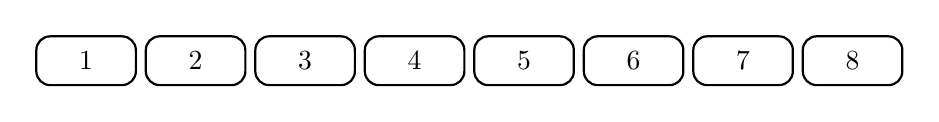
\begin{tikzpicture}

    \matrix[ng] (m) { & & & & & & & \\ } ;

    \node[cell, fit=(m-1-1)(m-1-1), inner sep=0pt, label=center: 1] {};
    \node[cell, fit=(m-1-2)(m-1-2), inner sep=0pt, label=center: 2] {};
    \node[cell, fit=(m-1-3)(m-1-3), inner sep=0pt, label=center: 3] {};
    \node[cell, fit=(m-1-4)(m-1-4), inner sep=0pt, label=center: 4] {};
    \node[cell, fit=(m-1-5)(m-1-5), inner sep=0pt, label=center: 5] {};
    \node[cell, fit=(m-1-6)(m-1-6), inner sep=0pt, label=center: 6] {};
    \node[cell, fit=(m-1-7)(m-1-7), inner sep=0pt, label=center: 7] {};
    \node[cell, fit=(m-1-8)(m-1-8), inner sep=0pt, label=center: 8] {};

  \end{tikzpicture}

\end{frame}

\begin{frame}[fragile]
  \centering

  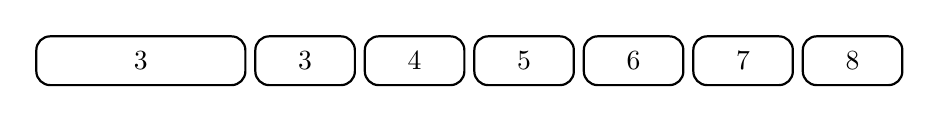
\begin{tikzpicture}

    \matrix[ng] (m) { & & & & & & & \\ } ;

    \node[cell, fit=(m-1-1)(m-1-2), inner sep=0pt, label=center: 3] {};
    \node[cell, fit=(m-1-3)(m-1-3), inner sep=0pt, label=center: 3] {};
    \node[cell, fit=(m-1-4)(m-1-4), inner sep=0pt, label=center: 4] {};
    \node[cell, fit=(m-1-5)(m-1-5), inner sep=0pt, label=center: 5] {};
    \node[cell, fit=(m-1-6)(m-1-6), inner sep=0pt, label=center: 6] {};
    \node[cell, fit=(m-1-7)(m-1-7), inner sep=0pt, label=center: 7] {};
    \node[cell, fit=(m-1-8)(m-1-8), inner sep=0pt, label=center: 8] {};

  \end{tikzpicture}

\end{frame}

\begin{frame}[fragile]
  \centering

  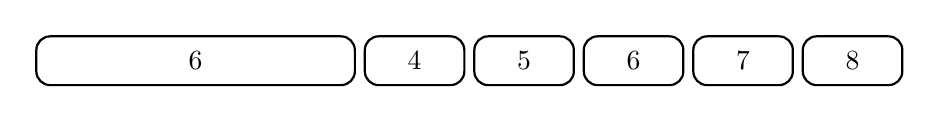
\begin{tikzpicture}

    \matrix[ng] (m) { & & & & & & & \\ } ;

    \node[cell, fit=(m-1-1)(m-1-3), inner sep=0pt, label=center: 6] {};
    \node[cell, fit=(m-1-4)(m-1-4), inner sep=0pt, label=center: 4] {};
    \node[cell, fit=(m-1-5)(m-1-5), inner sep=0pt, label=center: 5] {};
    \node[cell, fit=(m-1-6)(m-1-6), inner sep=0pt, label=center: 6] {};
    \node[cell, fit=(m-1-7)(m-1-7), inner sep=0pt, label=center: 7] {};
    \node[cell, fit=(m-1-8)(m-1-8), inner sep=0pt, label=center: 8] {};

  \end{tikzpicture}

\end{frame}

\begin{frame}[fragile]
  \centering

  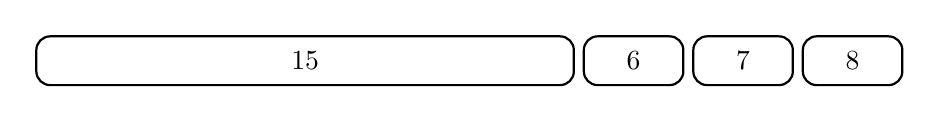
\begin{tikzpicture}

    \matrix[ng] (m) { & & & & & & & \\ } ;

    \node[cell, fit=(m-1-1)(m-1-5), inner sep=0pt, label=center: 15] {};
    \node[cell, fit=(m-1-6)(m-1-6), inner sep=0pt, label=center: 6]  {};
    \node[cell, fit=(m-1-7)(m-1-7), inner sep=0pt, label=center: 7]  {};
    \node[cell, fit=(m-1-8)(m-1-8), inner sep=0pt, label=center: 8]  {};

  \end{tikzpicture}

\end{frame}

\begin{frame}[fragile]
  \centering

  
\begin{tikzpicture}

    \matrix[ng] (m) { & & & & & & & \\ } ;

    \node[cell, fit=(m-1-1)(m-1-8), inner sep=0pt, label=center: 36] {};

  \end{tikzpicture}

\end{frame}

%%%%%%%%%%%%%%%%%%%%%%%%%%%%%%%%%%%%%%%%%%%%%%%%%%%%%%%%%%%%%%%%%%%%%%%%%%%%%%%
%% Parallel folding
%%%%%%%%%%%%%%%%%%%%%%%%%%%%%%%%%%%%%%%%%%%%%%%%%%%%%%%%%%%%%%%%%%%%%%%%%%%%%%%

\begin{frame}[fragile]
  \centering

  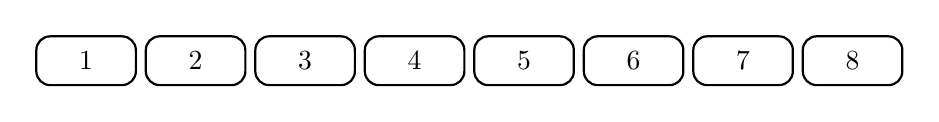
\begin{tikzpicture}

    \matrix[ng] (m) { & & & & & & & \\ } ;

    \node[cell, fit=(m-1-1)(m-1-1), inner sep=0pt, label=center: 1]  {};
    \node[cell, fit=(m-1-2)(m-1-2), inner sep=0pt, label=center: 2]  {};
    \node[cell, fit=(m-1-3)(m-1-3), inner sep=0pt, label=center: 3]  {};
    \node[cell, fit=(m-1-4)(m-1-4), inner sep=0pt, label=center: 4]  {};
    \node[cell, fit=(m-1-5)(m-1-5), inner sep=0pt, label=center: 5]  {};
    \node[cell, fit=(m-1-6)(m-1-6), inner sep=0pt, label=center: 6]  {};
    \node[cell, fit=(m-1-7)(m-1-7), inner sep=0pt, label=center: 7]  {};
    \node[cell, fit=(m-1-8)(m-1-8), inner sep=0pt, label=center: 8]  {};

  \end{tikzpicture}

\end{frame}

\begin{frame}[fragile]
  \centering

  
\begin{tikzpicture}

    \matrix[ng] (m) { & & & & & & & \\ } ;

    \node[cell, fit=(m-1-1)(m-1-2), inner sep=0pt, label=center: 3]  {};
    \node[cell, fit=(m-1-3)(m-1-4), inner sep=0pt, label=center: 7]  {};
    \node[cell, fit=(m-1-5)(m-1-6), inner sep=0pt, label=center: 11] {};
    \node[cell, fit=(m-1-7)(m-1-8), inner sep=0pt, label=center: 15] {};

  \end{tikzpicture}

\end{frame}

\begin{frame}[fragile]
  \centering

  
\begin{tikzpicture}

    \matrix[ng] (m) { & & & & & & & \\ } ;

    \node[cell, fit=(m-1-1)(m-1-4), inner sep=0pt, label=center: 10] {};
    \node[cell, fit=(m-1-5)(m-1-8), inner sep=0pt, label=center: 26] {};

  \end{tikzpicture}

\end{frame}

\begin{frame}[fragile]
  \centering

  
\begin{tikzpicture}

    \matrix[ng] (m) { & & & & & & & \\ } ;

    \node[cell, fit=(m-1-1)(m-1-8), inner sep=0pt, label=center: 36] {};

  \end{tikzpicture}

\end{frame}

%%%%%%%%%%%%%%%%%%%%%%%%%%%%%%%%%%%%%%%%%%%%%%%%%%%%%%%%%%%%%%%%%%%%%%%%%%%%%%%
%% Hierarchy
%%%%%%%%%%%%%%%%%%%%%%%%%%%%%%%%%%%%%%%%%%%%%%%%%%%%%%%%%%%%%%%%%%%%%%%%%%%%%%%

\begin{frame}[fragile]
  \centering

  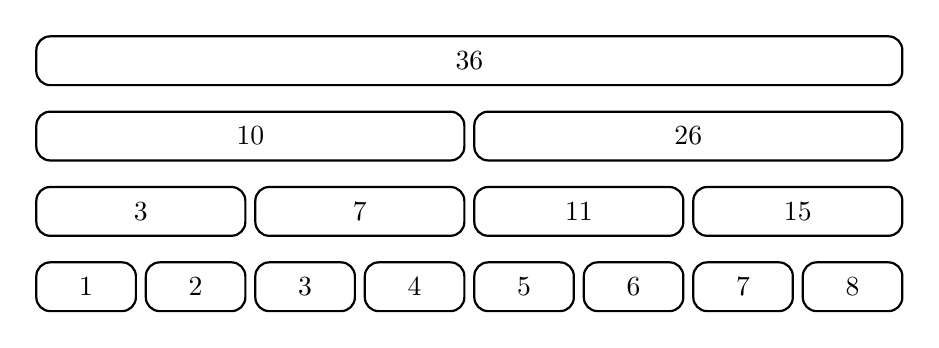
\begin{tikzpicture}

    \matrix[ng] (m) {
      & & & & & & & \\
      & & & & & & & \\
      & & & & & & & \\
      & & & & & & & \\
    } ;

    \node[cell, fit=(m-4-1)(m-4-1), inner sep=0pt, label=center: 1]  {};
    \node[cell, fit=(m-4-2)(m-4-2), inner sep=0pt, label=center: 2]  {};
    \node[cell, fit=(m-4-3)(m-4-3), inner sep=0pt, label=center: 3]  {};
    \node[cell, fit=(m-4-4)(m-4-4), inner sep=0pt, label=center: 4]  {};
    \node[cell, fit=(m-4-5)(m-4-5), inner sep=0pt, label=center: 5]  {};
    \node[cell, fit=(m-4-6)(m-4-6), inner sep=0pt, label=center: 6]  {};
    \node[cell, fit=(m-4-7)(m-4-7), inner sep=0pt, label=center: 7]  {};
    \node[cell, fit=(m-4-8)(m-4-8), inner sep=0pt, label=center: 8]  {};

    \node[cell, fit=(m-3-1)(m-3-2), inner sep=0pt, label=center: 3]  {};
    \node[cell, fit=(m-3-3)(m-3-4), inner sep=0pt, label=center: 7]  {};
    \node[cell, fit=(m-3-5)(m-3-6), inner sep=0pt, label=center: 11] {};
    \node[cell, fit=(m-3-7)(m-3-8), inner sep=0pt, label=center: 15] {};


    \node[cell, fit=(m-2-1)(m-2-4), inner sep=0pt, label=center: 10] {};
    \node[cell, fit=(m-2-5)(m-2-8), inner sep=0pt, label=center: 26] {};

    \node[cell, fit=(m-1-1)(m-1-8), inner sep=0pt, label=center: 36] {};

  \end{tikzpicture}

\end{frame}

\begin{frame}
  \centering
  \Large

  \textbf{Associative composition}
  allows for \textcolor{darkred}{modular}
  \textcolor{darkblue}{decomposition} and \textcolor{darkblue}{reasoning}.
\end{frame}

%%%%%%%%%%%%%%%%%%%%%%%%%%%%%%%%%%%%%%%%%%%%%%%%%%%%%%%%%%%%%%%%%%%%%%%%%%%%%%%
%% Composing programs
%%%%%%%%%%%%%%%%%%%%%%%%%%%%%%%%%%%%%%%%%%%%%%%%%%%%%%%%%%%%%%%%%%%%%%%%%%%%%%%

\begin{frame}[fragile]

  \frametitle{Composing programs}

  \centering
  \Large

  \begin{cminted}{scala}

A

  \end{cminted}

\end{frame}

\begin{frame}[fragile]

  \frametitle{Composing programs}

  \centering
  \Large

  \begin{cminted}{scala}

F[A]

  \end{cminted}

\end{frame}

\begin{frame}[fragile]

  \frametitle{Composing programs}

  \centering
  \Large

  \begin{cminted}{scala}

(F[A], F[A]) => F[A]

  \end{cminted}

\end{frame}

\begin{frame}[fragile]

  \frametitle{Composing programs}

  \centering
  \Large

  \begin{cminted}{scala}

(F[A], F[B]) => F[?]

  \end{cminted}

\end{frame}

\begin{frame}[fragile]

  \frametitle{Composing programs}

  \centering
  \Large

  \begin{cminted}{scala}

(F[A], F[B]) => F[(A, B)]

  \end{cminted}

\end{frame}

\begin{frame}[fragile]

  \frametitle{Composing programs}

  \begin{minted}{scala}

    def zipOption[A, B]
      (oa: Option[A], ob: Option[B]): Option[(A, B)] =

      (oa, ob) match {
        case (Some(a), Some(b)) => Some((a, b))
        case _                  => None
      }

  \end{minted}

\end{frame}

\begin{frame}[fragile]

  \frametitle{Composing programs}

  \begin{minted}{scala}

    def zipList[A, B]
      (la: List[A], lb: List[B]): List[(A, B)] =

      la match {
        case Nil    => Nil
        case h :: t => lb.map((h, _)) ++ zipList(t, f)
      }

  \end{minted}

\end{frame}

\begin{frame}[fragile]

  \frametitle{Composing programs}

  \begin{minted}{scala}

    def zipFunction[A, B, X]
      (f: X => A, g: X => B): X => (A, B) =

      (x: X) => (f(x), g(x))

  \end{minted}

\end{frame}

\begin{frame}[fragile]

  \begin{minted}{scala}

    trait Monoidal[F[_]] {
      def zip[A, B](fa: F[A], fb: F[B]): F[(A, B)]
      def pure[A](a: A): F[A]

      /*
      def map[A, B](fa: F[A])(f: A => B): F[B]
      */
    }

  \end{minted}

\end{frame}

\begin{frame}[fragile]

  \frametitle{Composing programs}
  \large

  \begin{itemize}
    \item $F(\rule{1ex}{.4pt})$: type of program \pause
    \item $\otimes: F(A) \times F(B) \rightarrow F((A, B))$ \pause
    \item $\eta: A \rightarrow F(A)$ \pause
  \end{itemize}

  $$(fa \otimes fb) \times fc \cong fa \times (fb \otimes fc)$$ \gpause
  $$fa \cong fa \otimes \eta_{Unit} \cong \eta_{Unit} \otimes fa$$

\end{frame}

\begin{frame}[fragile]

  \frametitle{Composing programs}

  \centering
  \Large

  \begin{cminted}{scala}

(F[A], F[B]) => F[(A, B)]

  \end{cminted}

\end{frame}

\begin{frame}[fragile]

  \frametitle{Composing independent programs}

  \centering
  \Large

  \begin{cminted}{scala}

(F[A], F[B]) => F[(A, B)]

  \end{cminted}

\end{frame}

\begin{frame}[fragile]

  \frametitle{Composing programs}

  \centering
  \Large

  \begin{cminted}{scala}

F[A]

  \end{cminted}

\end{frame}

%%%%%%%%%%%%%%%%%%%%%%%%%%%%%%%%%%%%%%%%%%%%%%%%%%%%%%%%%%%%%%%%%%%%%%%%%%%%%%%
%% Composing dependent programs
%%%%%%%%%%%%%%%%%%%%%%%%%%%%%%%%%%%%%%%%%%%%%%%%%%%%%%%%%%%%%%%%%%%%%%%%%%%%%%%

\begin{frame}[fragile]

  \frametitle{Composing dependent programs}

  \centering
  \Large

  \begin{cminted}{scala}

(F[A], A => F[B]) => F[B]

  \end{cminted}

\end{frame}

\begin{frame}[fragile]

  \frametitle{Composing dependent programs}

  \begin{minted}{scala}

    def flatMapOption[A, B]
      (oa: Option[A], f: A => Option[B]): Option[B] =

      oa match {
        case Some(a) => f(a)
        case None    => None
      }

  \end{minted}

\end{frame}

\begin{frame}[fragile]

  \frametitle{Composing dependent programs}

  \begin{minted}{scala}

    def flatMapList[A, B]
      (la: List[A], f: A => List[B]): List[B] =

      la match {
        case Nil => Nil
        case h :: t => f(h) ++ flatMapList(t, f)
      }

  \end{minted}

\end{frame}

\begin{frame}[fragile]

  \frametitle{Composing dependent programs}

  \begin{minted}{scala}

    def flatMapFunction[A, B, X]
      (fa: X => A, f: A => (X => B)): X => B =

      (x: X) => f(fa(x))(x)

  \end{minted}

\end{frame}

\begin{frame}[fragile]

  \begin{minted}{scala}

    trait Monad[F[_]] {
      def flatMap[A, B](fa: F[A])(f: A => F[B]): F[B]
      def pure[A](a: A): F[A]
    }

  \end{minted}

\end{frame}

\begin{frame}[fragile]

  \begin{minted}{scala}

    trait Monad[F[_]] extends Monoidal[F] {
      def flatMap[A, B](fa: F[A])(f: A => F[B]): F[B]
      def pure[A](a: A): F[A]
    }

  \end{minted}

\end{frame}

\begin{frame}

  \frametitle{Composing dependent programs}
  \large

  \begin{itemize}
    \item $F(\rule{1ex}{.4pt})$: type of program \pause
    \item $\bind: (F(A) \times A \rightarrow F(B)) \rightarrow F(B)$ \pause
    \item $\eta: A \rightarrow F(A)$ \pause
  \end{itemize}

  $$(fa \bind f) \bind g \ \ = \ \ fa \bind (f \kcomp g)\footnotemark$$ \gpause
  $$f(x) \ \ = \ \ \eta(x) \bind f$$ \gpause
  $$fa \ \ = \ \ fa \bind \eta$$

  \footnotetext[1]{$\kcomp: (A \rightarrow F(B) \times B \rightarrow F(C)) \rightarrow A \rightarrow F(C)$}

\end{frame}

\begin{frame}

  \frametitle{A nicer monad}
  \large

  $$f: A \rightarrow F(B)$$
  $$g: B \rightarrow F(C)$$
  $$h: C \rightarrow F(D)$$ \pause
  $$(f \kcomp g) \kcomp h \ \ = \ \ f \kcomp (g \kcomp h)$$ \gpause
  $$f \ \ = \ \ f \kcomp \eta \ \ = \ \ \eta \kcomp f$$

\end{frame}

%%%%%%%%%%%%%%%%%%%%%%%%%%%%%%%%%%%%%%%%%%%%%%%%%%%%%%%%%%%%%%%%%%%%%%%%%%%%%%%
%% Hierarchy 2
%%%%%%%%%%%%%%%%%%%%%%%%%%%%%%%%%%%%%%%%%%%%%%%%%%%%%%%%%%%%%%%%%%%%%%%%%%%%%%%

\begin{frame}[fragile]
  \centering

  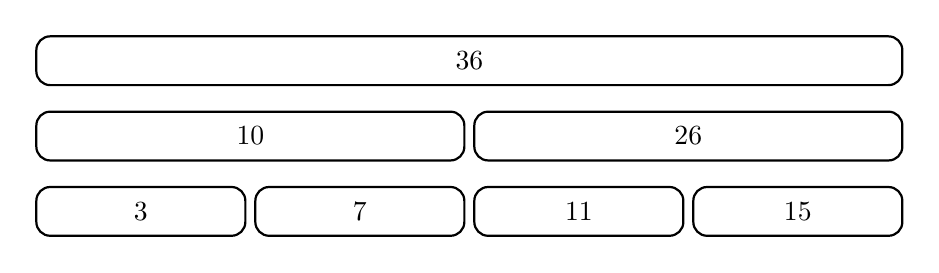
\begin{tikzpicture}

    \matrix[ng] (m) {
      & & & & & & & \\
      & & & & & & & \\
      & & & & & & & \\
    } ;

    \node[cell, fit=(m-3-1)(m-3-2), inner sep=0pt, label=center: 3]  {};
    \node[cell, fit=(m-3-3)(m-3-4), inner sep=0pt, label=center: 7]  {};
    \node[cell, fit=(m-3-5)(m-3-6), inner sep=0pt, label=center: 11] {};
    \node[cell, fit=(m-3-7)(m-3-8), inner sep=0pt, label=center: 15] {};


    \node[cell, fit=(m-2-1)(m-2-4), inner sep=0pt, label=center: 10] {};
    \node[cell, fit=(m-2-5)(m-2-8), inner sep=0pt, label=center: 26] {};

    \node[cell, fit=(m-1-1)(m-1-8), inner sep=0pt, label=center: 36] {};

  \end{tikzpicture}

\end{frame}

\begin{frame}[fragile]
  \centering

  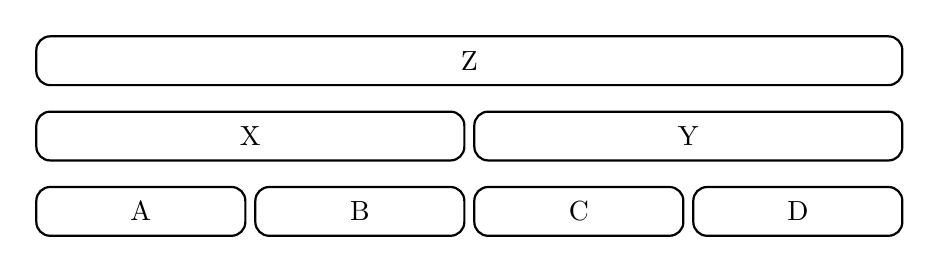
\begin{tikzpicture}

    \matrix[ng] (m) {
      & & & & & & & \\
      & & & & & & & \\
      & & & & & & & \\
    } ;

    \node[cell, fit=(m-3-1)(m-3-2), inner sep=0pt, label=center: A]  {};
    \node[cell, fit=(m-3-3)(m-3-4), inner sep=0pt, label=center: B]  {};
    \node[cell, fit=(m-3-5)(m-3-6), inner sep=0pt, label=center: C] {};
    \node[cell, fit=(m-3-7)(m-3-8), inner sep=0pt, label=center: D] {};


    \node[cell, fit=(m-2-1)(m-2-4), inner sep=0pt, label=center: X] {};
    \node[cell, fit=(m-2-5)(m-2-8), inner sep=0pt, label=center: Y] {};

    \node[cell, fit=(m-1-1)(m-1-8), inner sep=0pt, label=center: Z] {};

  \end{tikzpicture}

\end{frame}

\begin{frame}[fragile]
  \centering

  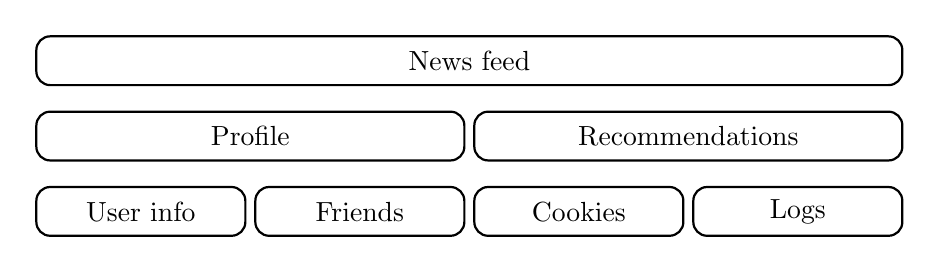
\begin{tikzpicture}

    \matrix[ng] (m) {
      & & & & & & & \\
      & & & & & & & \\
      & & & & & & & \\
    } ;

    \node[cell, fit=(m-3-1)(m-3-2), inner sep=0pt, label=center: User info]  {};
    \node[cell, fit=(m-3-3)(m-3-4), inner sep=0pt, label=center: Friends]  {};
    \node[cell, fit=(m-3-5)(m-3-6), inner sep=0pt, label=center: Cookies] {};
    \node[cell, fit=(m-3-7)(m-3-8), inner sep=0pt, label=center: Logs] {};


    \node[cell, fit=(m-2-1)(m-2-4), inner sep=0pt, label=center: Profile] {};
    \node[cell, fit=(m-2-5)(m-2-8), inner sep=0pt, label=center: Recommendations] {};

    \node[cell, fit=(m-1-1)(m-1-8), inner sep=0pt, label=center: News feed] {};

  \end{tikzpicture}

\end{frame}

%%%%%%%%%%%%%%%%%%%%%%%%%%%%%%%%%%%%%%%%%%%%%%%%%%%%%%%%%%%%%%%%%%%%%%%%%%%%%%%
%% Category theory
%%%%%%%%%%%%%%%%%%%%%%%%%%%%%%%%%%%%%%%%%%%%%%%%%%%%%%%%%%%%%%%%%%%%%%%%%%%%%%%

\begin{frame}
  \centering
  \large

  \textbf{Category theory}
  studies the algebra of composition.
\end{frame}

\begin{frame}

  \frametitle{Category theory}
  \large

  \begin{itemize}
    \item objects: A, B, C ... \pause
    \item arrows: $f: A \rightarrow B$, $g: B \rightarrow C$ ... \pause
    \item $1_{A}: A \rightarrow A$ \pause
  \end{itemize}

  $$(f \circ g) \circ h = f \circ (g \circ h)$$ \gpause
  $$f = f \circ 1_{A} = 1_{A} \circ f$$

\end{frame}

\begin{frame}[fragile]
  \centering
  \frametitle{Category theory}
  \Large

  \begin{tikzcd}
    & B \arrow[dr, "g"] \\
    A \arrow[ur, "f"] \arrow[rr, "g \circ f"'] && C
  \end{tikzcd}

\end{frame}

\begin{frame}[fragile]
  \centering
  \frametitle{Category theory: monoids}
  \Large

  \begin{tikzcd}
    & \bullet \arrow[out=210, in=150, loop, distance=3.0cm, "x"]           % left
              \arrow[out=120, in=60,  loop, distance=3.0cm, "y"]           % top
              \arrow[out=30,  in=-30, loop, distance=3.0cm, "x \oplus y"]  % right
  \end{tikzcd}

\end{frame}

\begin{frame}[fragile]
  \centering
  \frametitle{Category theory: monoids}
  \Large

  \begin{tikzcd}
    & \bullet \arrow[out=210, in=150, loop, distance=3.0cm, "x"]           % left
              \arrow[out=120, in=60,  loop, distance=3.0cm, "y"]           % top
              \arrow[out=30,  in=-30, loop, distance=3.0cm, "x \oplus y"]  % right
              \arrow[out=300, in=240, loop, distance=3.0cm, "1_{A}"]       % bottom
  \end{tikzcd}

\end{frame}

\begin{frame}[fragile]
  \centering
  \frametitle{Category theory: monads}
  \Large

  \pause

  \begin{tikzcd}
    & F(B) \\
    A \arrow[ur, "f"] \arrow[rr, "? \circ f"'] && F(C)
  \end{tikzcd}

  \pause

  $$\bind: (F(A) \times A \rightarrow F(B)) \rightarrow F(B)$$

\end{frame}

\begin{frame}[fragile]
  \centering
  \frametitle{Category theory: monads}
  \Large

  \begin{tikzcd}
    & F(B) \\
    A \arrow[ur, "f"] \arrow[rr, "? \circ f"'] && F(C)
  \end{tikzcd}

  $$\bind: (A \rightarrow F(B)) \rightarrow F(A) \rightarrow F(B)$$

\end{frame}

\begin{frame}[fragile]
  \centering
  \frametitle{Category theory: monads}
  \Large

  \begin{tikzcd}
    & F(B) \arrow[dr, "g^{*}"] \\
    A \arrow[ur, "f"] \arrow[rr, "g^{*} \circ f"'] && F(C)
  \end{tikzcd}

  $$\bind: (A \rightarrow F(B)) \rightarrow F(A) \rightarrow F(B)$$

\end{frame}

\begin{frame}[fragile]
  \centering
  \frametitle{Category theory: monads}
  \Large

  \begin{tikzcd}
    & B \arrow[dr, dashrightarrow, "g'"] \\
    A \arrow[ur, dashrightarrow, "f'"] \arrow[rr, dashrightarrow, "g' \circ f'"'] && C
  \end{tikzcd}

\end{frame}

\begin{frame}[fragile]
  \centering
  \frametitle{Category theory: monads}
  \Large

  \begin{tikzcd}
    & B \arrow[dr, dashrightarrow, "g'"] \arrow[out=120, in=60, loop, dashrightarrow, distance=1.0cm, "1_{B}"] \\
    A \arrow[ur, dashrightarrow, "f'"] \arrow[rr, dashrightarrow, "g' \circ f'"']
      \arrow[out=300, in=240, loop, dashrightarrow, distance=1.0cm, "1_{A}"]
    && C \arrow[out=300, in=240, loop, dashrightarrow, distance=1.0cm, "1_{C}"]
  \end{tikzcd}

\end{frame}

\begin{frame}[fragile]
  \centering
  \frametitle{Category theory: monads}
  \Large

  \begin{tikzcd}
    & B \arrow[dr, dashrightarrow, "g'"] \arrow[out=120, in=60, loop, dashrightarrow, distance=1.0cm, "B \rightarrow T(B)"] \\
    A \arrow[ur, dashrightarrow, "f'"] \arrow[rr, dashrightarrow, "g' \circ f'"']
      \arrow[out=300, in=240, loop, dashrightarrow, distance=1.0cm, "A \rightarrow T(A)"]
    && C \arrow[out=300, in=240, loop, dashrightarrow, distance=1.0cm, "C \rightarrow T(C)"]
  \end{tikzcd} \pause

  $$\eta: A \rightarrow F(A)$$

\end{frame}

%%%%%%%%%%%%%%%%%%%%%%%%%%%%%%%%%%%%%%%%%%%%%%%%%%%%%%%%%%%%%%%%%%%%%%%%%%%%%%%
%% Compose composers
%%%%%%%%%%%%%%%%%%%%%%%%%%%%%%%%%%%%%%%%%%%%%%%%%%%%%%%%%%%%%%%%%%%%%%%%%%%%%%%

\begin{frame}
  \centering
  \large

  Can we compose the composers?
\end{frame}

\begin{frame}[fragile]

  \centering
  \Large

  \begin{cminted}{scala}

(A, A) => A

  \end{cminted}

\end{frame}

\begin{frame}[fragile]

  \centering
  \large

  \begin{cminted}{scala}

(Monoid[A], Monoid[B]) => Monoid[?]

  \end{cminted}

\end{frame}

\begin{frame}[fragile]

  \frametitle{Product composition: monoids}
  \centering
  \large

  \begin{cminted}{scala}

(Monoid[A], Monoid[B]) => Monoid[(A, B)]

  \end{cminted}

\end{frame}

\begin{frame}[fragile]

  \frametitle{Product composition: monoids}
  \footnotetext{Assuming \code{Monoid[A]} and \code{Monoid[B]}}

  \begin{minted}{scala}
def append(x: (A, B), y: (A, B)): (A, B) = {
  val a = x._1 append y._1
  val b = x._2 append y._2

  (a, b)
}
  \end{minted}

  \pause

  \begin{minted}{scala}
def empty: (A, B) = (Monoid[A].empty, Monoid[B].empty)
  \end{minted}

\end{frame}

\begin{frame}[fragile]

  \centering
  \large

  \begin{cminted}{scala}

(F[A], F[B]) => F[(A, B)]

  \end{cminted}

\end{frame}

\begin{frame}[fragile]

  \centering
  \large

  \begin{cminted}{scala}

(Monoidal[F], Monoidal[G]) => Monoidal[?]

  \end{cminted}

\end{frame}

\begin{frame}[fragile]

  \frametitle{Product composition: lax monoidal functors}
  \centering
  \large

  \begin{cminted}{scala}

type L[X] = (F[X], G[X])
(Monoidal[F], Monoidal[G]) => Monoidal[L]

  \end{cminted}

\end{frame}

\begin{frame}[fragile]

  \frametitle{Product composition: lax monoidal functors}
  \footnotetext{Assuming \code{Monoidal[F]} and \code{Monoidal[G]}}

  \begin{minted}{scala}
def zip[A, B](x: (F[A], G[A]),
              y: (F[B], G[B])): (F[(A, B)], G[(A, B)]) = {

  val f = x._1 zip y._1
  val g = x._2 zip y._2

  (f, g)
}
  \end{minted}

  \pause

  \begin{minted}{scala}
def pure[A](a: A): (F[A], G[A]) =
  (Monoidal[F].pure(a), Monoidal[G].pure(a))
  \end{minted}

\end{frame}

\begin{frame}[fragile]

  \frametitle{Product composition: monads}
  \centering
  \large

  \begin{cminted}{scala}

type L[X] = (F[X], G[X])
(Monad[F], Monad[G]) => Monad[L]

  \end{cminted}

\end{frame}

\begin{frame}[fragile]

  \frametitle{Product composition: monads}
  \footnotetext{Assuming \code{Monad[F]} and \code{Monad[G]}}

  \begin{minted}{scala}
def flatMap[A, B]
  (xa: (F[A], G[A]))(ff: A => (F[B], G[B])):
    (F[(A, B)], G[(A, B)]) = {

  val f = xa._1.flatMap(a => ff(a)._1)
  val g = xa._2.flatMap(a => ff(a)._2)

  (f, g)
}
  \end{minted}

\end{frame}

\begin{frame}[fragile]

  \frametitle{Nested composition: lax monoidal functors}
  \centering
  \large

  \begin{cminted}{scala}

type L[X] = F[G[X]]
(Monoidal[F], Monoidal[G]) => Monoidal[L]

  \end{cminted}

\end{frame}

\begin{frame}[fragile]

  \frametitle{Nested composition: lax monoidal functors}
  \footnotetext{Assuming \code{Monoidal[F]} and \code{Monoidal[G]}}

  \begin{minted}{scala}
def zip[A, B](fga: F[G[A]], fgb: F[G[B]]): F[G[(A, B)]] = {
  val fp: F[(G[A], G[B])] = fga zip fgb
  fp.map { case (ga, gb) => ga zip gb }
}
  \end{minted}

  \pause

  \begin{minted}{scala}
def pure[A](a: A): F[G[A]] =
  Monoidal[F].pure(Monoidal[G].pure(a))
  \end{minted}

\end{frame}

\begin{frame}[fragile]

  \frametitle{Nested composition: monads}
  \centering
  \large

  \begin{cminted}{scala}

type L[X] = F[G[X]]
(Monad[F], Monad[G]) => Monad[L]

  \end{cminted}

\end{frame}

\begin{frame}[fragile]

  \frametitle{Nested composition: monads}
  \centering
  \large

  \begin{cminted}{scala}

type L[X] = F[G[X]]
(Monad[F], Monad[G]) => Monad[L]

  \end{cminted}
  
\begin{tikzpicture}[overlay]
    \draw[red, very thick] (-8, 1) -- (1, -0.5);
    \draw[red, very thick] (-8, -0.5) -- (1, 1);
  \end{tikzpicture}

\end{frame}

\begin{frame}[fragile]

  \frametitle{Nested composition: monads}
  \footnotetext{Assuming \code{Monad[F]} and \code{Monad[G]}}

  \begin{minted}{scala}
def flatMap[A, B](fga: F[G[A]](f: A => F[G[B]]): F[G[B]] =
  \end{minted}

  \pause

  \begin{minted}{scala}
  fga.flatMap { (ga: G[A]) =>
    ???
  }
  \end{minted}

\end{frame}

\begin{frame}

  \frametitle{Review}
  \large

  \begin{itemize}
    \item Associative composition allows for modular decomposition and reasoning \pause
    \item Monoids compose A's, lax monoidal functors compose independent F[A]'s, monads compose dependent F[A]'s \pause
    \item Monoids can be composed \pause
    \item Lax monoidal functors can be composed \pause
    \item Monads in general cannot be composed
  \end{itemize}

\end{frame}

\begin{frame}

  \frametitle{References}

  \begin{itemize}
    \item Equational reasoning at scale - Gabriel Gonzalez
      \url{http://www.haskellforall.com/2014/07/equational-reasoning-at-scale.html}
    \item Invariant Shadows - Michael Pilquist
      \url{http://mpilquist.github.io/blog/2015/06/22/invariant-shadows-part-2/}
    \item All About Applicative - Me!
      \url{https://www.youtube.com/watch?v=Mn7BtPALFys}
    \item A Categorial View of Computational Effects - Prof. Emily Riehl
      \url{https://www.youtube.com/watch?v=6t6bsWVOIzs}
    \item Conceptual Mathematics - F. William Lawvere and Stephen H. Schanuel
  \end{itemize}

\end{frame}

\end{document}
